%%%%%%%%%%%%%%%%%%%%%%%%%%%%%%%%%%%%%%%%%%%%%%%%%%%%%%%%%%%%%%%%%%%%%%%%%%%%%%%%%%%%
% Document data
%%%%%%%%%%%%%%%%%%%%%%%%%%%%%%%%%%%%%%%%%%%%%%%%%%%%%%%%%%%%%%%%%%%%%%%%%%%%%%%%%%%%
\documentclass[12pt]{article} %report allows for chapters
%%%%%%%%%%%%%%%%%%%%%%%%%%%%%%%%%%%%%%%%%%%%%%%%%%%%%%%%%%%%%%%%%%%%%%%%%%%%%%%%%%%%
\usepackage{preamble}
\usepackage{caption}
\usepackage{subcaption}
\newcommand{\innprod}[2]{\left\langle #1, #2\right\rangle}
\newcommand{\blade}[1]{\boldsymbol{\vec{#1}}}

\begin{document}

\begin{center}
   \textsc{\large MATH 272, Homework 6, \emph{Solutions}}\\
\end{center}
\vspace{.5cm}


\begin{problem} \textbf{(11 pts)} Are you sure you understand what constitutes a vector space? What about an inner product? Let's see a few examples. Please work through each part of the question.

Given an a vector space $V$ with an inner product $\innprod{-}{-}$, we can always define a \emph{norm} (or \emph{energy}) by taking $v\in V$ and putting
\[
\|v\|^2 = \innprod{v}{v}.
\]
\emph{P.S. both l's seen here are short for Henri Lebesgue.}
\begin{enumerate}[(a)]
\item \textbf{(3 pts)} (Finite dimensional inner product space) Consider the vector space $\C^3$ with the Hermitian inner product $\innprod{-}{-}$.
\begin{itemize}
\item Compute the norm of 	
\[
		\vecu = \begin{pmatrix} i \\ 1 \\ 0 \end{pmatrix}.
	\]
\item Compute the norm of
\[
\vecv = \begin{pmatrix} 1 \\ -i \\ 0 \end{pmatrix}.
\]
\item Compute the inner product $\innprod{\vecu}{\vecv}$.
\item Provide an example of a basis for $\C^3$. 
\end{itemize}

\item \textbf{(4 pts)} (Countably infinite dimensional inner product space) Consider the space of \emph{square summable} (\emph{finite energy}) sequences $\ell^2(\C)$. That is, an element of the $\ell^2(\C)$ is a sequence of complex numbers $\{a_n\}_{n=0}^\infty$ with an inner product defined by
\[
\innprod{\{a_n\}}{\{b_n\}} = \sum_{n=0}^\infty a_n^* b_n.
\]
and we require the vectors to have finite energy which gives us the definition:
\[
\ell^2(\C) \coloneqq \{ \{a_n\} ~|~ a_n \in \C ~\textrm{such that $\|\{a_n\}\|<\infty$}\}.
\]
\begin{itemize}
\item Show that the sequence $a_n = \frac{1}{n+1}$ is in $\ell^2(\C)$. What is its norm? \emph{Please use WolframAlpha!}
\item Show that the sequence $b_n = \frac{1}{2^n}$ is in $\ell^2(\C)$. What is its norm? 
\item Compute the inner product $\innprod{\{a_n\}}{\{b_n\}}$. \emph{Please use WolframAlpha!}
\item Provide an example of a basis for $\ell^2(\C)$.
\end{itemize}

\item \textbf{(4 pts)} (Functional inner product space) Consider the space of \emph{square integrable} (\emph{finite energy}) functions $L^2(\Omega)$ on the region $\Omega=[0,1]$. That is, an element of the $L^2(\Omega)$ is a complex-valued function $f \colon [0,1] \to \C$ of complex numbers with an inner product defined by
\[
\innprod{f}{g} = \int_\Omega f^*g d\Omega = \int_0^1 f^*(x) g(x)dx.
\]
and we require the vectors to have finite energy which gives us the definition:
\[
L^2(\Omega) \coloneqq \{ f\colon \Omega \to \C ~|~ \textrm{such that $\|f\|<\infty$}\}.
\]
\begin{itemize}
\item Show that the function $f(x)= e^{i2\pi x}$ is in $L^2(\Omega)$. What is its norm? 
\item Show that the sequence $g(x) = \sin(2\pi x)$ is in $L^2(\Omega)$. What is its norm?
\item Compute the inner product $\innprod{f}{g}$. \emph{Please use WolframAlpha!}
\end{itemize}
\end{enumerate}
\end{problem}
\begin{solution}~
\begin{enumerate}[(a)]
\item Let us do each part here:
\begin{itemize}
\item First, the norm of $\vecu$ is
\[
		\innprod{\vecu}{\vecu} = \sum_{j=1}^3 u_j^* u_j =  i^* \cdot i +1\cdot 1 + 0\cdot 0 = 2.
\]
\item Second, 
\[
		\innprod{\vecv}{\vecv} = \sum_{j=1}^3 v_j^* v_j =  1^* \cdot 1 + (-i)^*\cdot (-i) + 0\cdot 0 = 2.
\]
\item Their inner product is
\[
	\innprod{\vecu}{\vecv} = \sum_{j=1}^3 u_j^* v_j =  i^* \cdot 1 + 1 \cdot (-i) + 0\cdot 0 = 0.
\]

\item A basis is a linearly independent spanning set. Hence, one choice is the set of vectors
\[
\blade{e}_1 = \begin{pmatrix} 1 \\ 0 \\ 0 \end{pmatrix} \qquad \blade{e}_2 = \begin{pmatrix} 0 \\ 1 \\ 0 \end{pmatrix} \qquad \blade{e}_3 = \begin{pmatrix} 0 \\ 0 \\ 3 \end{pmatrix}.
\]
This is because any vector $\blade{w}$ in $\C^3$ can be written as a linear combination
\[
\blade{w} = \sum_{j=1}^3 \alpha_j \blade{e}_j
\]
where $\alpha_j \in \C$.
\end{itemize}
\item Let us do each part here:
\begin{itemize}
\item First, the norm of $\{a_n\}$ is
\[
		\innprod{\{a_n\}}{\{a_n\}} = \sum_{n=1}^\infty a_n^* a_n = \sum_{n=1}^\infty \frac{1}{(n+1)^2} = \frac{\pi^2}{6}.
\]
Since this norm is finite, $\{a_n\} \in \ell^2(\C)$. We have actually seen this series before in a previous homework.
\item Second, 
\[
			\innprod{\{b_n\}}{\{b_n\}} = \sum_{n=1}^\infty b_n^* b_n = \sum_{n=1}^\infty \frac{1}{2^{2n}} = \frac{4}{3}.
\]
\item Their inner product is
\[
		\innprod{\{a_n\}}{\{b_n\}} = \sum_{n=1}^\infty a_n^* b_n = \sum_{n=1}^\infty \frac{1}{2^n (n+1)} = \ln(4),
\]
where $\ln$ is the natural log. Since this norm is finite, $\{a_n\} \in \ell^2(\C)$. A bit weird, huh? Can you figure out what $\ln(x)$ would be? You've actually done this before.

\item A basis is a linearly independent spanning set. Hence, one choice is the set of sequences
\[
\{e_0\} = 1,0,0,0\dots \qquad \{e_1\} = 0,1,0,0,\dots \qquad \{e_j\} = 0,0,0,\dots,0,1,0,\dots
\]
for all $j=0,1,2,3,\dots$ and where $\{e_j\}$ is the sequence that whose $j$th term is $1$ and all other terms are zero. 
This is because any vector (sequence) $\{c_n\}$ in $\ell^2(\C)$ can be written as a linear combination
\[
\{c_n\} = \sum_{j=0}^\infty \alpha_j \{e_j\}
\]
where $\alpha_j \in \C$.
\end{itemize}

\item Let us do each part here:
\begin{itemize}
\item First, the norm of $f$ is
\[
		\innprod{f}{f} = \int_0^1 f^* f dx = \int_0^1 e^{-i2\pi x} e^{i2\pi x} dx = \int_0^1 1 dx = 1.
\]
Since this integral is finite, $f\in L^2(\Omega)$ for $\Omega = [0,1]$.
\item Second, 
\[
			\innprod{g}{g} = \int_0^1 g^* g dx = \int_0^1 \sin(2\pi x)^2 dx =  \frac{1}{2}.
\]
Since this integral is finite, $f\in L^2(\Omega)$ for $\Omega = [0,1]$.
\item Their inner product is
\[
		\innprod{f}{g} = \int_0^1 f^* g dx = \int_0^1 e^{-i2\pi x}*\sin(2\pi x) dx =  \frac{1}{2}i.
\]
Can you see why you get $\frac{1}{2} i$ using Euler's formula?
\end{itemize}
\end{enumerate}
\end{solution}
\vspace*{1cm}
\textcolor{red}{
\noindent \textbf{Rubric:}
\begin{enumerate}[(a)]
    \item \textbf{(1 pt.)} Correct norms. \textbf{(1 pt.)} Correct inner product. \textbf{(1 pt.)} Student provided a working basis.
    \item \textbf{(1 pt.)} Correct norm for $a_n$. \textbf{(1 pt.)} Correct norm for $a_n$ \textbf{(1 pt.)} Correct inner product. \textbf{(1 pt.)} Some kind of working basis or an explanation of what it would look like.
    \item \textbf{(2 pt.)} Correct norm for $f$. \textbf{(2 pt.)} Correct norm for $g$ \textbf{(BONUS 1 pt.)} Correct inner product. I typoed this on the original problem, so don't mark it wrong if the student did this incorrectly.
\end{enumerate}
}

\newpage
\begin{problem} \textbf{(4 pts)} Consider the real function $f(x)=1 \in L^2(\Omega)$ on the domain $\Omega = [0,L]$.
	\begin{enumerate}[(a)]
		\item \textbf{(1 pts)} What is the norm of $f$, $\|f\|$?
		\item \textbf{(1 pts)} Normalize $f(x)$.
		\item \textbf{(2 pts)} Find a nonzero normalized polynomial of degree $\leq 1$ that is orthogonal to $f(x)$.
	\end{enumerate}
\end{problem}
\begin{solution}~
	\begin{enumerate}[(a)]
		\item We compute the norm by
		\begin{align*}
			\|f\| = \sqrt{\innprod{f}{f}} &=\sqrt{ \int_0^L f^2(x)dx}\\
			&=\sqrt{ \int_0^L 1 dx}\\
			&= \sqrt{L}.
		\end{align*}
		\item We can normalize $f$ by letting $c$ be some constant and forcing
		\[
		1=\|cf\| = c^2L.
		\]
		Thus $c=\frac{1}{\sqrt{L}}$.  We can write the normalized function as
		\[
		h(x)=\frac{1}{\sqrt{L}}. 
		\]
		\item Consider an arbitrary polynomial of degree $\leq 1$ by putting $g(x)=ax+b$.  Now, we want this polynomial to be orthogonal to $f(x)$ which means that we want
		\[
		\innprod{f}{g}=0.
		\]
		Let us compute the above
		\begin{align*}
			\innprod{f}{g} &= \int_0^L f(x)g(x)dx\\
			&=\int_0^L ax+bdx\\
			&= \frac{aL^2}{2}+bL\\
			&= \frac{1}{2}L\left(aL+2b\right).
		\end{align*}
		Hence, we can solve for $a$ by
		\[
		0=aL+2b \quad \implies \quad a= -\frac{2b}{L}.
		\]
		Now, $g(x)=-\frac{2b}{L}x+b$.  But, we require $g(x)$ to be normalized as well hence
		\begin{align*}
			1=\innprod{g}{g} &= \int_0^L \left(-\frac{2b}{L}x+b\right)^2dx\\
			&= \frac{b^2L}{3}.
		\end{align*}
		Solving for $b$, we find $b=\sqrt{\frac{3}{L}}$ and hence we have that
		\[
		g(x) = -2\sqrt{\frac{3}{L^3}}x+\sqrt{\frac{3}{L}}..
		\]
	\end{enumerate}
\end{solution}
\vspace*{1cm}
\textcolor{red}{
\noindent \textbf{Rubric:}
\begin{enumerate}[(a)]
    \item \textbf{(1 pt.)} Correct norm and shown work.
    \item \textbf{(1 pt.)} Correct normalization.
    \item \textbf{(2 pt.)} Right idea for work shown. \textbf{(1 pt.)} Correct answer (there may be more than one!).
\end{enumerate}
}

\newpage
\begin{problem}
\textbf{(6 pts)} A wavefunction $\Psi$ for a particle in the 1-dimensional box $\Omega=[0,1]$ is a member of the space of finite energy functions $L^2(\Omega)$. Recall that $\Psi$ could be written as a superposition of normalized states
	\[
	\psi_n(x) = \sqrt{2} \sin\left(n\pi x\right).
	\]
	That is,
	\[
	\Psi(x) = \sum_{n=1}^\infty a_n \psi_n(x),
	\]
	for some choice of the coefficients $a_n$.
	\begin{enumerate}[(a)]
		\item \textbf{(3 pts)} Let $a_n = \frac{\sqrt{6}}{n\pi}$. Show that $\Psi(x)$ is normalized. \emph{Hint: first, use orthogonality of the states $\psi_n(x)$ to your advantage. Then you will need to know what an infinite series evaluates to. Use a tool like WolframAlpha to evaluate this series.}
		\item \textbf{(2 pts)} Note that we can approximate $\Psi(x)$ by taking a finite sum approximation up to some chosen $N$ by
		\[
			\Psi(x) \approx \sum_{n=1}^N a_n \psi_n(x).
		\]
		Plot the approximation of $\Psi(x)$ for $N=1,5,25,50,100$.  
\item \textbf{(1 pts)} Describe the wave function $\Psi$.
		\end{enumerate}
\end{problem}
\begin{solution}
	\begin{enumerate}[(a)]
		\item To see that $\Psi(x)$ is normalized we take
		\begin{align*}
			\innprod{\Psi}{\Psi} &= \innprod{\sum_{n=1}^\infty a_n \psi_n(x)}{\sum_{n=1}^\infty a_n \psi_n(x)}\\
			&= \sum_{n=1}^\infty \|a_n\|^2 \innprod{\psi_n}{\psi_n} &\textrm{by orthogonality of the states}\\
			&= \sum_{n=1}^\infty \frac{6}{n^2 \pi^2}\\
			&= \frac{6}{\pi^2} \sum_{n=1}^\infty \frac{1}{n^2}\\
			&= \frac{6}{\pi^2} \zeta(2)\\
			&= 1.
		\end{align*}
		Note the sum above is what appeared in Problem 1 also. It has to do with the Zeta function we saw in Math 271 and $\zeta(2)$ is a well-known value (that you can find by computing the above sum in, for example, WolframAlpha).
		\item ~
	\begin{figure}[H]
	\centering
		\begin{subfigure}[h]{0.48\textwidth}
			\centering
			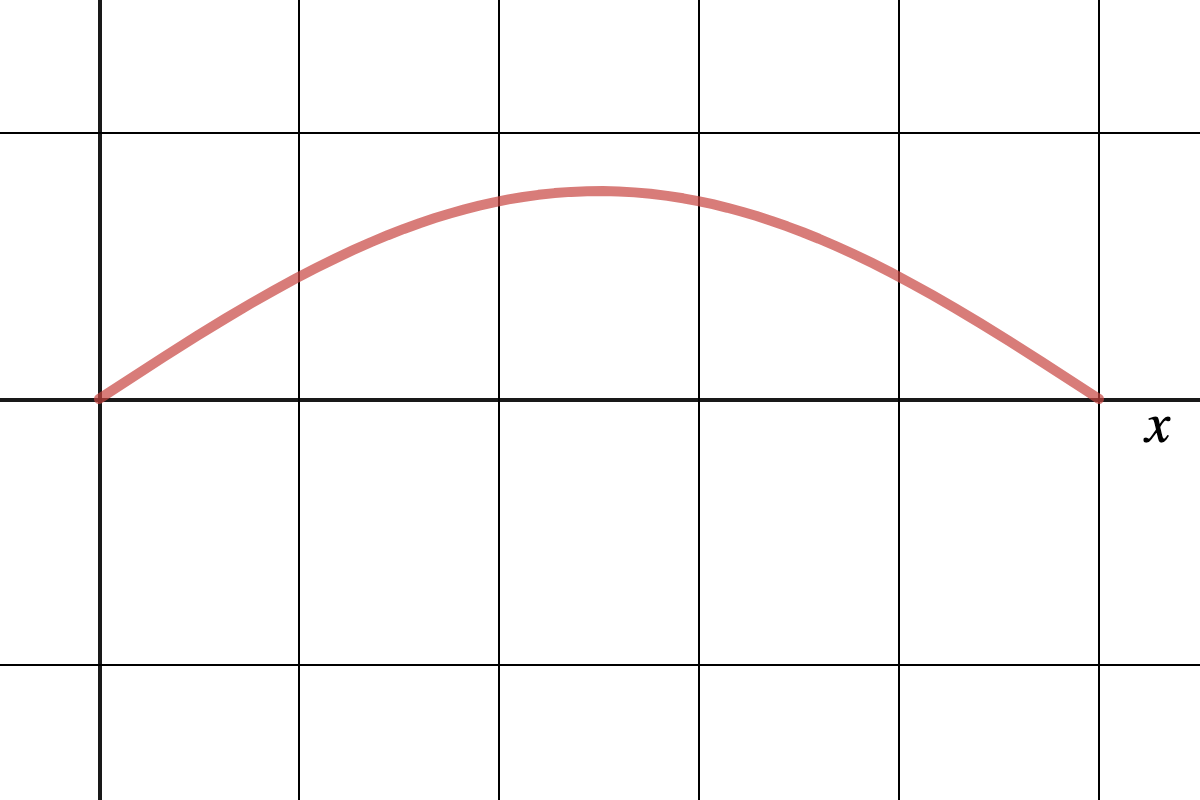
\includegraphics[width=.8\textwidth]{figures/n=1.png}
			\caption{The approximation to $\Psi(x)$ with $N=1$.}
		\end{subfigure}
		~
		\begin{subfigure}[h]{0.48\textwidth}
			\centering
			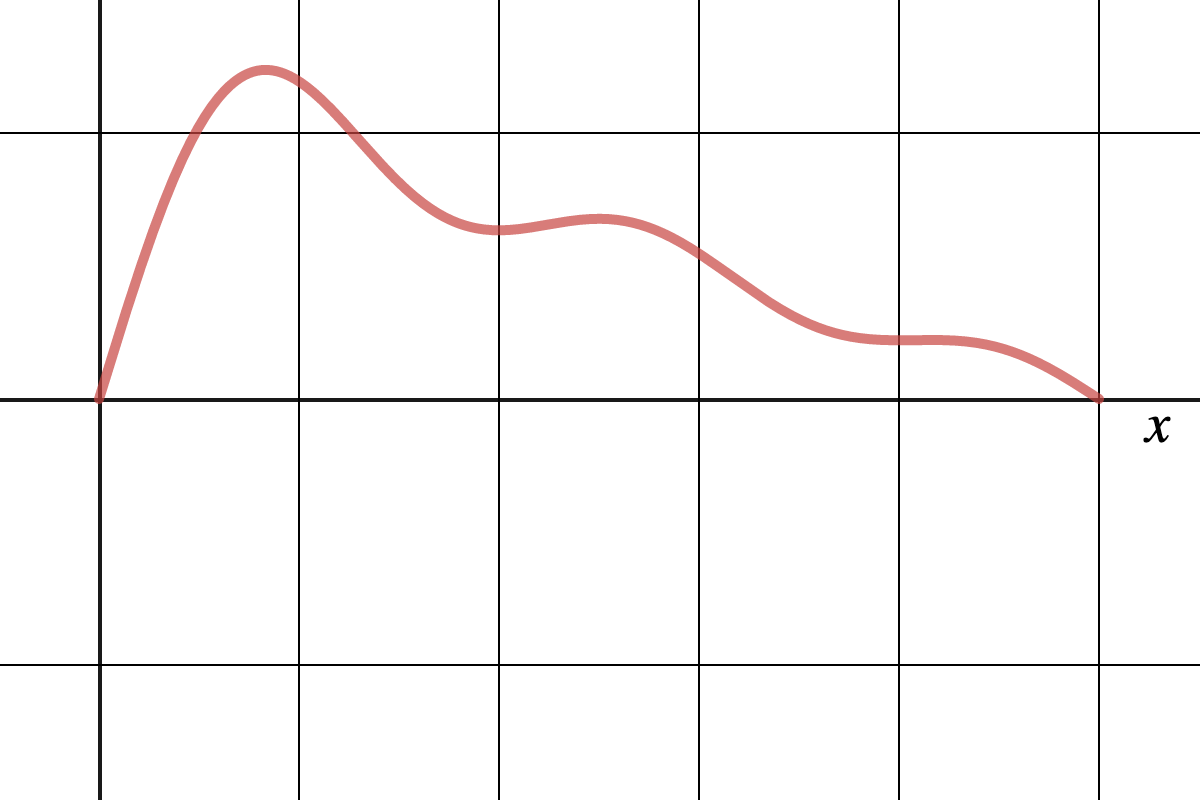
\includegraphics[width=.8\textwidth]{figures/n=5.png}
			\caption{The approximation to $\Psi(x)$ with $N=5$.}
		\end{subfigure}
		\\
		\begin{subfigure}[h]{0.48\textwidth}
			\centering
			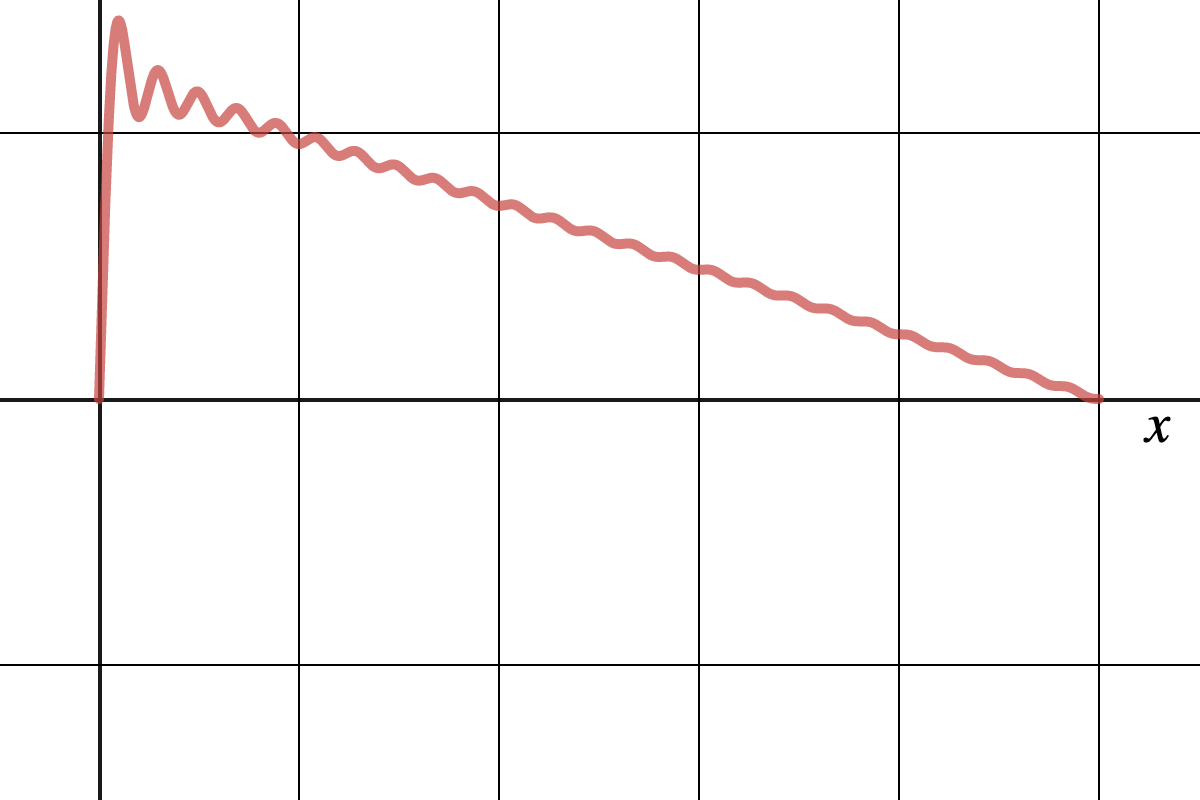
\includegraphics[width=.8\textwidth]{figures/n=50.png}
			\caption{The approximation to $\Psi(x)$ with $N=50$.}
		\end{subfigure}
		~
		\begin{subfigure}[h]{0.48\textwidth}
			\centering
			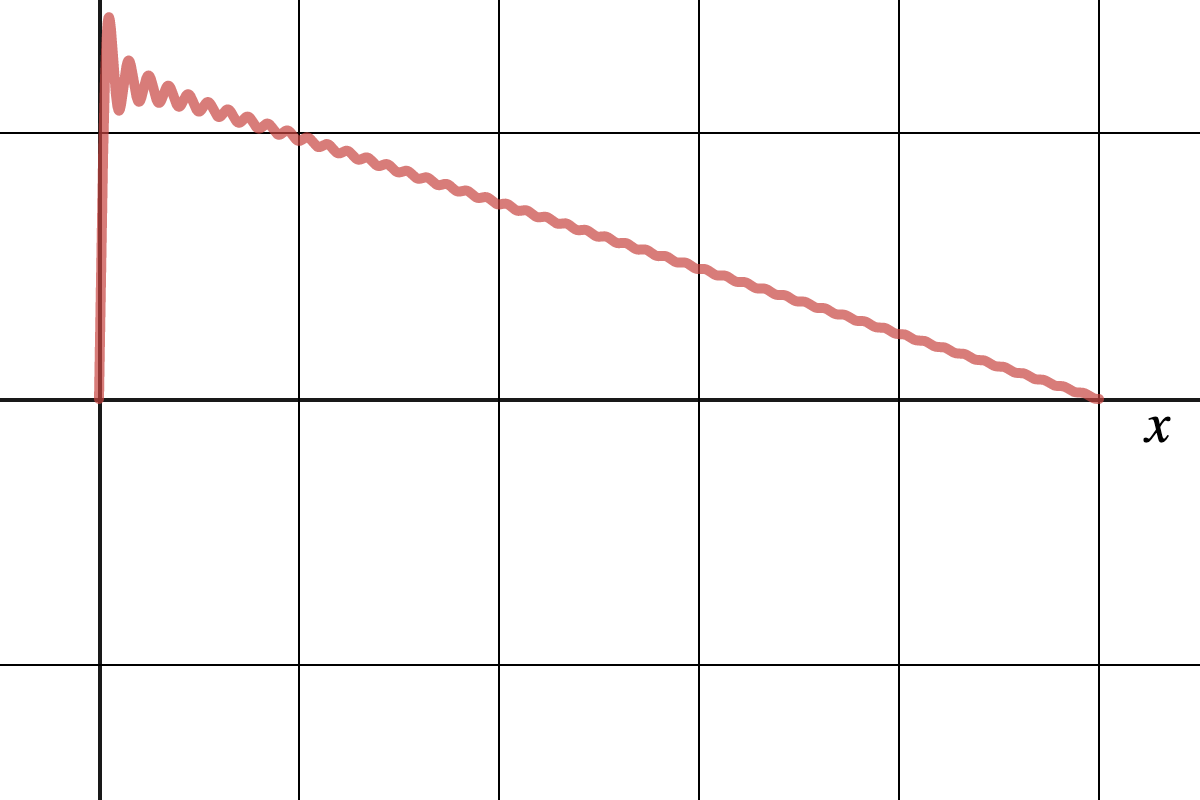
\includegraphics[width=.8\textwidth]{figures/n=100.png}
			\caption{The approximation to $\Psi(x)$ with $N=100$.}
		\end{subfigure}
	\end{figure}
	\end{enumerate}
\item The wave function seems to approach a straight line solution that has a discontinuous jump at $x=0$. This is because we do require $\Psi(0)=0=\Psi(1)$. The probability will be concentrated more towards $x=0$ and decrease linearly as $x$ approaches 1.
\end{solution}
\vspace*{1cm}
\textcolor{red}{
\noindent \textbf{Rubric:}
\begin{enumerate}[(a)]
    \item \textbf{(1 pt.)} Correct starting point to find the norm. \textbf{(1 pt.)} Simplifies work to get a single sum. \textbf{(1 pt.)} Evaluates the sum to get 1 showing the wavefunction is normalized.
    \item \textbf{(1 pt.)} Approximations are graphed in the correct domain. \textbf{(1 pt.)} One approximation for each of the given values (can be on the same graph).
    \item \textbf{(1 pt.)} Basically, remark the wave function approaches a straight line. Ideally, student mentions that the boundary conditions are still satisfied.
\end{enumerate}
}

\newpage
\begin{problem}
\textbf{(9 pts)}  When making a measurement of the position of the particle, we will use the \emph{position operator} $x$.  This is the same as the variable $x$ in the original problem statement, but it is also an operator! Similarly, we could measure the momentum of a particle using the \emph{momentum operator $p$}. The potential $V(x)$ is a function of the position operator and it, itself, is an operator. Lastly, I should mention the \emph{Hamiltonian operator} $H=\frac{p^2}{2M} + V$. 

What I mean here by operator is that the operators defined above are linear transformations $\mathcal{L} \colon L^2(\Omega) \to L^2(\Omega)$. \emph{Actually, I am lying to you. It is true that $x\colon L^2(\Omega) \to L^2(\Omega)$ but you have to be careful which spaces you are talking about when it comes to the momentum operator $p$. Do not worry, this understanding that the underlying space is $L^2(\Omega)$ is good enough!}
   \begin{enumerate}[(a)]
		\item \textbf{(1 pts)} True or false. A self-adjoint operator has a real-valued spectrum.
   		\item \textbf{(1 pts)} Show that the position operator $x$ is self-adjoint.
   		\item \textbf{(2 pts)} We can compute the expected position of a particle with wavefunction $\Psi(x)$ by computing
   		\[
   		\mathbb{E}[x]=\innprod{\Psi}{x\Psi}.
   		\]
   		Let $\Psi(x) = \psi_1(x)$, compute $\mathbb{E}[x]$. This value $\mathbb{E}[x]$ tells you where we expect to find the particle on average. 
        \item \textbf{(1 pts)} In fact, any real valued function $V(x)$ of the position operator $x$ is also self-adjoint. Make a quick argument on why this must be true.
		\item \textbf{(2 pts)} We define the \emph{momentum operator} $p = -i\hbar \frac{d}{dx}$. Using integration by parts, show that this operator is self-adjoint.
		\item \textbf{(2 pts)} Argue that the Hamiltonian operator is self-adjoint. \emph{Hint: look at how $H$ is defined. Don't show more work than you need to. This part should be short and sweet.}
   	\end{enumerate}
\end{problem}
\begin{remark}
The fact that all measurements in quantum mechanics are self-adjoint operators motivates the Dirac bra-ket notation which looks like this:
\[
\mathbb{E}[x] = \langle \Psi \vert ~x~ \vert \Psi \rangle.
\]
This is because $x$ can act on either side!
\end{remark}
\begin{solution}~
	\begin{enumerate}[(a)]
		\item True! This is a theorem we had before in class.
		\item Let $\Psi(x)$ and $\Phi(x)$ be arbitrary functions.  Then we have
		\begin{align*}
			\innprod{x\Psi}{\Phi} &= \int_0^L x \Psi(x)\Phi^*(x)dx\\
			&= \int_0^1 \Psi(x) \left(x \Phi(x)\right)^*dx &\textrm{since $x$ is real valued}\\
			&= \innprod{\Psi}{x\Phi}.
		\end{align*}
		Thus we have that the position operator is self-adjoint.
		\item We can compute the expected value by
		\begin{align*}
			\mathbb{E}[x] = \innprod{\Psi}{x\Psi} &= \int_0^L \Psi(x) x^* \Psi(x)dx\\
			&= \int_0^1 x\psi_1(x)^2dx\\
			&= 2\int_0^1 x \sin(\pi x)^2 dx\\
			&= \frac{1}{2}.
		\end{align*}
		Hence, you expect to find the particle at $x=\frac{1}{2}$ most often.
        \item If $V(x)$ is real valued, then $V^*(x)=V(x)$.  Hence, we have
	\[
	\innprod{V\Psi}{\Phi} = \int_0^1 V(x)\Psi(x)\Phi^*(x)dx = \int_0^1 \Psi(x)\left(V(x)\Phi(x)\right)^*dx = \innprod{\Psi}{V\Phi}.
	\]
	\item We have
\begin{align*}
	\innprod{p \Psi}{\Phi} &= \int_0^L \left(-i\hbar \frac{d \Psi}{dx}\right)\Phi^*(x)dx\\
	&= \left.-i\hbar \Psi(x)\Phi^*(x)  \right\vert_0^1 + \int_0^1 i\hbar \Psi(x) \frac{d\Phi^*}{dx}dx & \textrm{by integration by parts}.
\end{align*}
Note now that the boundary conditions require both $\Psi(0)=\Psi(1)=0$ and $\Phi(0)=\Phi(1)=0$, since we are working over the space of solutions to the particle in the 1-dimensional box.  Hence, we have
\begin{align*}
	\innprod{p\Psi}{\Phi} &= \int_0^1 i\hbar \Psi(x) \frac{d\Phi^*}{dx}dx\\
	&= \int_0^1 \Psi(x)\left(-i\hbar \frac{d\Phi}{dx}\right)^* dx \\
	&= \innprod{\Psi}{p\Phi}.
\end{align*}
Thus, $p$ is Hermitian.

\item Note that the Hamiltonian operator is given by
\[
H=\frac{p^2}{2m} + V
\]
and so
\begin{align*}
	\innprod{H \Psi}{\Phi} &= \innprod{\left(\frac{p^2}{2m} + V\right) \Psi}{\Phi}\\
	&= \frac{1}{2m}\innprod{p^2 \Psi}{\Phi} + \innprod{ V \Psi}{\Phi}\\
	&= \frac{1}{2m}\innprod{p\Psi}{p\Phi} + \innprod{\Psi}{V \Phi}\\
	&= \innprod{\Psi}{\frac{p^2}{2m} \Phi} + \innprod{\Psi}{V \Phi}\\
	&= \innprod{\Psi}{H \Phi},
\end{align*}
so $H$ is self-adjoint.
	\end{enumerate}
\end{solution}
\vspace*{1cm}
\textcolor{red}{
\noindent \textbf{Rubric:}
\begin{enumerate}[(a)]
    \item \textbf{(1 pt.)} Correct answer with some reasoning.
    \item \textbf{(1 pt.)} Correct work and answer.
    \item \textbf{(1 pt.)} Correct work. \textbf{(1 pt.)} Correct final answer.
	\item \textbf{(1 pt.)} A short and reasonable argument.
	\item \textbf{(1 pt.)} Correct usage of integration by parts. \textbf{(1 pt.)} Use boundary conditions and get the correct final answer.
	\item \textbf{(1 pt.)} Write out $H$ in terms of momentum operator and potential. \textbf{(1 pt.)} Use the logic from previous parts of the problem or some other correct work.
\end{enumerate}
}

\newpage
\begin{problem}
\textbf{(6 pts)} Let's explore two subspaces of $L^2(\Omega)$ for $\Omega = [0,1]$. One built by exponentials and one built by sines and cosines.
	\begin{enumerate}[(a)]
		\item \textbf{(3 pts)} Show that the set of functions $\{1,\sqrt{2}\cos(2n \pi x), \sqrt{2}\sin(2n \pi x)\}$ for integers $n\geq 1$ are orthonormal in $L^2(\Omega)$ with $\Omega = [0,1]$.
		\item \textbf{(3 pts)} Recall Euler's formula: $e^{ix} = \cos(x)+i\sin(x)$.  Argue that 
\[
\operatorname{Span}\{e^{i2n\pi x} ~|~ n \in \Z\} \qquad \textrm{and} \qquad \operatorname{Span}\{1,\sqrt{2}\cos(2n \pi x), \sqrt{2}\sin(2n \pi x) ~|~ n \in \Z, ~ n\geq 1\}
\]
are the same subspace. \emph{Hint: can you just show that a given $e^{i2n\pi x}$ corresponds to a pair $\cos(2n \pi x)$ and $\sin(2n \pi x)$ using Euler's formula? Also, you should use the fact that sine is an odd function and cosine is an even function.}
	\end{enumerate}
\end{problem}
\begin{solution}
\begin{enumerate}[(a)]
\item This just requires that we show the work for a few inner products. First,
\[
\innprod{1}{1} = \int_0^1 1^* 1 dx = \int_0^1 1 dx = 1,
\]
which shows 1 is normalized. Then
\begin{align*}
\innprod{1}{\sqrt{2} \sin(2n\pi x)} = \sqrt{2} \int_0^1 \sin(2n\pi x) dx = 0
\end{align*}
shows that $1$ is orthogonal to $\sin(2n \pi x)$ for any integer $n$ and
\begin{align*}
\innprod{1}{\sqrt{2} \cos(2n\pi x)} = \sqrt{2} \int_0^1 \cos(2n\pi x) dx = 0
\end{align*}
shows that $1$ is orthogonal to $\cos(2n \pi x)$ for any integer $n$.

Now, 
\[
\innprod{\sqrt{2}\cos(2m\pi x)}{\sqrt{2}\cos(2n\pi x)} = 2 \int_0^1 \cos(2m\pi x) \cos(2n\pi x) dx = \delta_{mn},
\]
where $\delta_{mn}$ is the Kronecker delta which is 1 if and only if $m=n$ and is otherwise zero. This shows $\sqrt{2}\cos(2m\pi x)$ is normalized and is otherwise orthogonal to the other cosine functions with $m\neq n$. Then
\begin{align*}
\innprod{\sqrt{2}\cos(2m\pi x)}{\sqrt{2} \sin(2n\pi x)} = 2 \int_0^1 \cos(2m\pi x)\sin(2n\pi x) dx = 0
\end{align*}
shows that $\sqrt{2}\cos(2m\pi x)$ is orthogonal to $\sin(2n \pi x)$ for any pair of integers $m$ and $n$. 

Finally, 
\[
\innprod{\sqrt{2}\sin(2m\pi x)}{\sqrt{2}\sin(2n\pi x)} = 2 \int_0^1 \sin(2m\pi x) \sin(2n\pi x) dx = \delta_{mn},
\]
This shows $\sqrt{2}\sin(2m\pi x)$ is normalized and is otherwise orthogonal to the other sine functions with $m\neq n$. 

All of the above work shows that the collection is orthonormal.

\item First, a function in $\operatorname{Span}\{e^{i2n\pi x} ~|~ n \in \Z\}$ is given by
\[
f(x) = \sum_{n=-\infty}^\infty c_n e^{i2n \pi x}.
\]
Now, we just use Euler's formula and work out the details by
\begin{align*}
\sum_{n=-\infty}^\infty c_n e^{i2n \pi x} &= c_0 + \sum_{n=-\infty}^{-1} c_n e^{i2n \pi x} + \sum_{n=1}^\infty c_n e^{i2n \pi x} \\
&= c_0 + \sum_{n=-\infty}^{-1} c_n (\cos(2n\pi x) + i \sin(2n\pi x)) + \sum_{n=1}^{\infty} c_n (\cos(2n\pi x) + i \sin(2n\pi x))\\
&= c_0 + \sum_{n=1}^{\infty} c_{-n} (\cos(-2n\pi x) + i \sin(-2n\pi x)) + \sum_{n=1}^{\infty} c_n (\cos(2n\pi x) + i \sin(2n\pi x)).
\end{align*}
The above was just manipulating the sums and realizing that $e^{0}=1$. Now, let us use the fact that cosine is an even function and sine is an odd function so that we have
\begin{align*}
f(x) &= c_0 + \sum_{n=1}^{\infty} c_{-n} (\cos(-2n\pi x) + i \sin(-2n\pi x)) + \sum_{n=1}^{\infty} c_n (\cos(2n\pi x) + i \sin(2n\pi x))\\
&= c_0 + \sum_{n=1}^{\infty} c_{-n} (\cos(2n\pi x) - i \sin(-2n\pi x)) + \sum_{n=1}^{\infty} c_n (\cos(2n\pi x) + i \sin(2n\pi x))
\end{align*}
then we can rearrange the terms into sums of cosines and sines by
\begin{align*}
f(x) &= c_0 + \sum_{n=1}^{\infty} c_{-n} (\cos(2n\pi x) - i \sin(-2n\pi x)) + \sum_{n=1}^{\infty} c_n (\cos(2n\pi x) + i \sin(2n\pi x))\\
&= c_0 + \sum_{n=1}^\infty (c_{n}+c_{-n})\cos(2n\pi x) + \sum_{n=1}^\infty i(c_n-c_{-n}) \sin(2n\pi x).
\end{align*}

Now we are basically done since a function in $\operatorname{Span}\{1,\sqrt{2}\cos(2n \pi x), \sqrt{2}\sin(2n \pi x) ~|~ n \in \Z, ~ n\geq 1\}$ is given by
\[
f(x) = c_0 + \sum_{n=1}^\infty a_n \cos(2n\pi x) + \sum_{n=1}^\infty b_n \sin(2n\pi x).
\]
Hence, $a_n = c_n + c_{-n}$ and $b_n = i(c_n - c_{-n})$ allows us to transform from the complex Fourier series representation to the one with cosines and sines!
\end{enumerate}
\end{solution}
\vspace*{1cm}
\textcolor{red}{
\noindent \textbf{Rubric:}
\begin{enumerate}[(a)]
    \item \textbf{(1 pt.)} Norm of 1 and 1 orthogonal to sines and cosines. \textbf{(1 pt.)} Norm of cosines and orthogonal to other cosines and all sines.  \textbf{(1 pt.)} Norm of sines and orthogonal to other sines and all cosines. 
	\item \textbf{(1 pt.)} Note that the idea of span is to take a linear combination (series in this case). \textbf{(1 pt.)} Showing some work to turn one series into the other using Euler's formula. \textbf{(1 pt.)} Whole process is correct and in the end there is some relationship of $a_n$ and $b_n$ in terms of $c_n$.
\end{enumerate}
}

\newpage
\begin{problem}
\textbf{(10 pts)} It turns out that the set of complex exponentials $\{e^{i2n\pi x} ~|~ n\in \Z\}$ is an orthonormal basis for $L^2(\Omega)$ for $\Omega = [0,1]$ (and thus by the previous problem, so are the sines and cosines). This is the foundational insight of the Fourier transform/series. Let us denote by $\phi_n(x) = e^{i2n\pi x}$.

Let $f \in L^2(\Omega)$, then the \emph{Fourier transform} of $f$ is the function $\hat{f} \colon \Z \to \C$ defined by
\[
\hat{f}(n) = \innprod{f}{\phi_n}.
\]
Then the \emph{Fourier series of $f$} is the series
\[
f(x) = \sum_{n=-\infty}^\infty \hat{f}(n) \phi_n(x)
\]
\begin{enumerate}[(a)]
\item \textbf{(2 pts)} Let $V$ be an $n$-dimensional vector space. Recall that you can write a vector $v \in V$ in terms of an orthonormal basis $v_1,\dots,v_n$ for $V$ by
\[
v = \sum_{j=1}^n \langle v,v_j\rangle v_j.
\]
Explain why the Fourier series is the same concept just for an infinite dimensional vector space.
\item \textbf{(2 pts)} Compute the Fourier transform of the function 
\[
f(x) = \begin{cases} 0, & 0\leq x \leq \frac{1}{4} \\
	1, &  \frac{1}{4} \leq x \leq \frac{3}{4} \\
 0, & \frac{3}{4}\leq x \leq 1 \end{cases}
\]
\emph{Please note that you will want to consider the term $\hat{f}(0)$ separately from the others.}
\item \textbf{(1 pts)} Write out the Fourier series of $f$. 
\item \textbf{(2 pts)} Convert the Fourier series of $f$ into a series of sine and cosine functions using Euler's formula. \emph{Hint: you can also just use this from the beginning and put}
\[
\hat{f}(n) = \langle f,\phi_n\rangle = \int_0^1 f(x)\cos(2n\pi x) dx + i \int_0^1 f(x)\sin(2n\pi x)dx.
\]
\item \textbf{(2 pts)} Plot an approximation of the Fourier series of sine and cosine functions up to $N=1,3,5,10,50,100$ only on the domain $\Omega$. Please graph your approximations to the original $f$. Describe what is happening with your approximations.
\item \textbf{(1 pts)} What happens if you plot your Fourier series over all of $\R$?
\end{enumerate}
\end{problem}
\begin{solution}
\begin{enumerate}[(a)]
\item Since we can write a Fourier series as
\[
f(x) = \sum_{n=-\infty}^\infty \hat{f}(n) \phi_n(x) = \sum_{n=-\infty}^\infty \innprod{f}{\phi_n} \phi_n(x),
\]
we see that this is really the same form. It's just our sum is now infinite as is our basis $\phi_n$.
\item First, let us find 
\[
c_0 = \hat{f}(0) = \innprod{f}{1} = \int_0^1 f dx = \int_\frac{1}{4}^\frac{3}{4} 1 dx = \frac{1}{2}.
\]
Note that is is actually just the average value of $f$ and that is what this term always is! Now, for $n\neq 0$ we have
\[
c_n = \hat{f}(n) = \innprod{f}{\phi_n} = \int_0^1 f e^{i2n\pi x} dx = \int_\frac{1}{4}^\frac{3}{4} e^{i2n\pi x} dx = \frac{e^{i \pi n}\sin\left(\frac{n \pi}{2}\right)}{\pi n} = \frac{(-1)^n\sin\left(\frac{n \pi}{2}\right) }{\pi n}.
\]
Our function $\hat{f} \colon \Z \to \C$ is our Fourier transform.

\item The Fourier series is 
\[
f(x) = \sum_{n=-\infty} \hat{f}(n) \phi_n(x) = \sum_{n=-\infty}^\infty  \frac{(-1)^n\sin\left(\frac{n \pi}{2}\right) }{\pi n} e^{i2n\pi x}.
\]

\item I will use the conversion found in Problem 5 so that
\[
a_n = c_n + c_{-n} = \frac{(-1)^n\sin\left(\frac{n \pi}{2}\right) }{\pi n} + \frac{(-1)^n\sin\left(\frac{-n \pi}{2}\right) }{\pi(-n)} = 2\frac{(-1)^n\sin\left(\frac{n \pi}{2}\right) }{\pi n}
\]
and
\[
b_n = i(c_n - c_{-n}) = i\left(\frac{(-1)^n\sin\left(\frac{n \pi}{2}\right) }{\pi n} - \frac{(-1)^n\sin\left(\frac{-n \pi}{2}\right) }{\pi (-n)}\right) = 0.
\]
\item Here is a plot of all the approximations of the function at once. 
\begin{figure}[H]
\centering
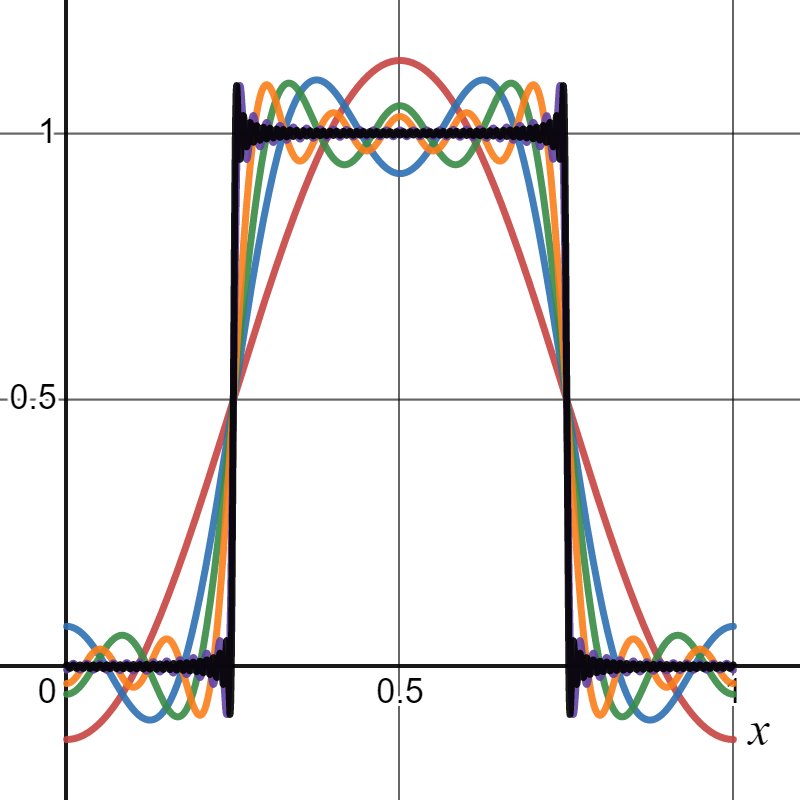
\includegraphics[width=0.5\textwidth]{figures/fourier_series.png}
\caption{Red curve is $N=1$, blue curve is $N=3$, green curve is $N=5$, orange curve is $N=10$, purple curve is $N=50$, and the black curve is $N=100$.}
\end{figure}
As $N$ increases, the approximations become closer to the original function $f(x)$. There is a jump at each point when the function is discontinuous, i.e., at $x=\frac{1}{4}$ and $x=\frac{3}{4}$.
\item Here is a plot where I don't restrict the domain of the Fourier series.
\begin{figure}[H]
\centering
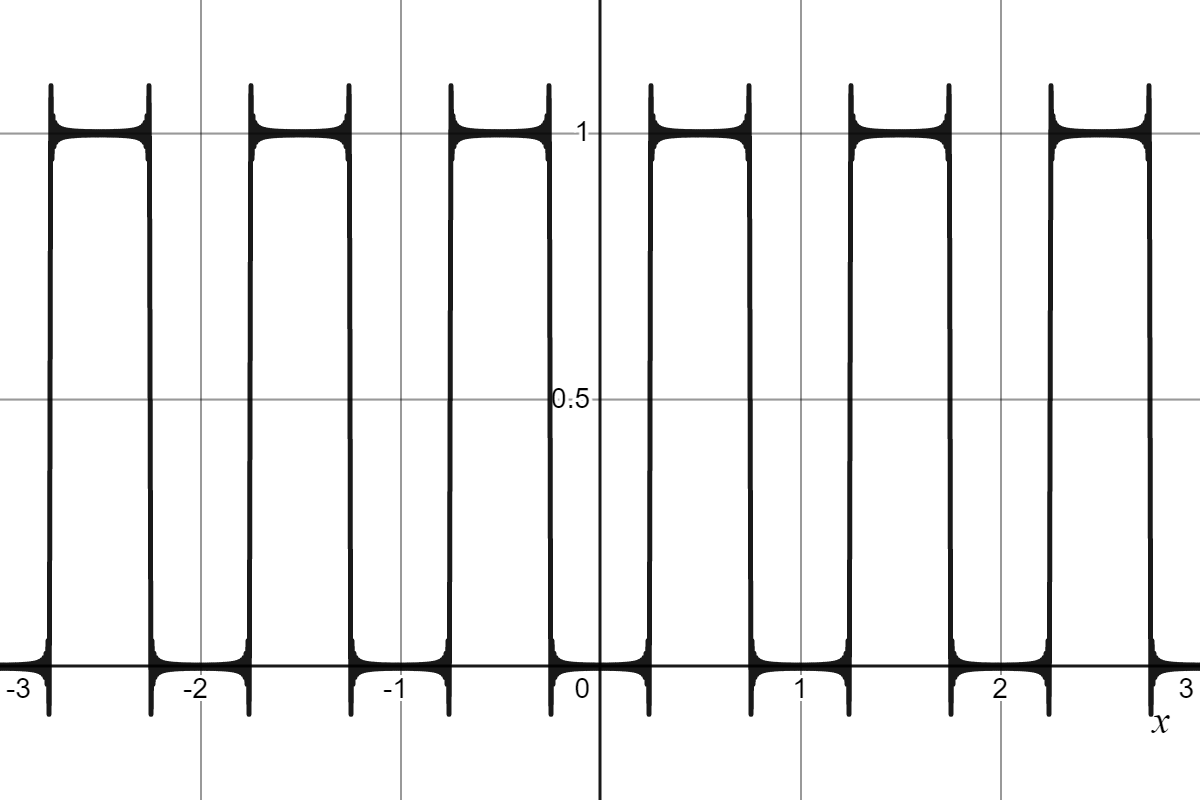
\includegraphics[width=0.75\textwidth]{figures/fourier_series_on_R.png}
\caption{Plotting just the $N=100$ case with no domain restriction.}
\end{figure}
Now we see that we have turned the function $f(x)$ defined only on $[0,1]$ into a periodic function on all of $\R$ using this technique.
\end{enumerate}
\end{solution}
\vspace*{1cm}
\textcolor{red}{
\noindent \textbf{Rubric:}
\begin{enumerate}[(a)]
    \item \textbf{(1 pt.)} A good explanation. \textbf{(1 pt.)} Write out the Fourier series using the inner product to show it looks the same.
	\item \textbf{(1 pt.)} Set up the correct integral. \textbf{(1 pt.)} Correct result from integral and correct $\hat{f}(0)$.
	\item \textbf{(1 pt.)} Correct Fourier series.
	\item \textbf{(1 pt.)} Some work to show how the student is going to convert from one to the other. \textbf{(1 pt.)} Correct conversion to cosine and sine. 
	\item \textbf{(1 pt.)} All approximations are plotted. \textbf{(1 pt.)} Describing that the series tends towards the original function. It would be good to also mention what happens at the discontinuities but it isn't required.
	\item \textbf{(1 pt.)} Explanation of what the Fourier series looks like when the domain isn't restricted. A plot could be helpful.
\end{enumerate}
}

\newpage
\begin{problem}
\textbf{(10 pts)} One advantage of the Fourier transform is that we can use it to solve differential equations in a new way that also allows us to consider far more general forcing terms. The basic idea is that the Fourier transform converts a differential equation into an algebraic equation. Let us see how this works.

First, let me say that we will be working over $L^2(\Omega)$ with $\Omega = [0,1]$. Recall the Dirac delta $\delta(x)$ which satisfies the properties
\[
\int_0^1 \delta(x-x_0) dx = 1 \qquad \textrm{and} \qquad \int_0^1 \delta(x-x_0) f(x) dx = f(x_0)
\]
whenever $x_0 \in \Omega$. You can imagine the Dirac delta $\delta(x- x_0)$ as a probability distribution where all the mass is located at a single point $x_0$.
\begin{enumerate}[(a)]
\item \textbf{(2 pts)} Show that for any $f$ satisfying the Dirichlet boundary conditions $f(0)=0$ and $f(1)=0$ that for $n\neq 0$
\[
\left\langle \frac{d}{dx} f , \phi_n \right\rangle = -i2 \pi n \hat{f}(n).
\]
\emph{Hint: use integration by parts.}
\item \textbf{(2 pts)} Consider the Poisson (elastic deformation) problem
\[
\begin{cases}
\frac{d^2}{dx^2} f(x) = \delta(x-x_0) \\
f(0)=0=f(1) & \textrm{as boundary conditions.}
\end{cases}
\]
Apply the Fourier transform to both sides to show that we have for $n\neq 0$
\[
\hat{f}(n) =  -\frac{e^{i2n\pi x_0}}{4\pi^2 n^2}.
\]
\item \textbf{(2 pts)} Hence, the solution to the problem is just the Fourier series
\[
f(x)=c_0 + c_1 x + \sum_{n=-\infty}^{-1} -\frac{e^{in \pi x_0}}{4\pi^2 n^2} \phi_n + \sum_{n=1}^\infty -\frac{e^{in \pi x_0}}{4\pi^2 n^2} \phi_n.
\]
Let $x_0=1/2$ and convert this Fourier series to a real valued Fourier series in terms of sines and cosines. 
\item \textbf{(1 pts)} Determine the constants $c_0$ and $c_1$ using the boundary conditions on $f$.
\item \textbf{(2 pts)} Plot your approximation to the Fourier series for $N=1,3,5,10,50,100$. 
\item \textbf{(1 pts)} Explain your result given the following interpretation: You can imagine that $\delta(x-1/2)$ is a point mass of mass 1 placed exactly at $x=1/2$ on your elastic rod $\Omega$. \emph{Hint: does this look what what you'd imagine the deformation to look like?}
\end{enumerate}
\end{problem}
\begin{solution}
\begin{enumerate}[(a)]
\item We have
\begin{align*}
\left\langle \frac{d}{dx} f , \phi_n \right\rangle &= \int_0^1 \frac{df}{dx} \phi_n(x) dx \\
&= f(x)\phi_n(x) \vert_0^1 - \int_0^1 f(x) \frac{d \phi_n}{dx} dx\\
&= 0 - \int_0^1 f(x) \frac{d}{dx} e^{i2n \pi x} dx
\end{align*}
by using the Dirichlet boundary values $f(0)=0=f(1)$. Then
\begin{align*}
\left\langle \frac{d}{dx} f , \phi_n \right\rangle &= -\int_0^1 f(x) \frac{d}{dx} e^{i2n \pi x} dx\\
&= -i2\pi n \int_0^1 f(x) e^{i2 n \pi x}dx\\
&= -i2 \pi n \hat{f}(n).
\end{align*}
\item Now, I will denote $\delta_{x_0}=\delta(x-x_)$ and we just use our result from (a) to help us so we apply the Fourier transform $\mathcal{F}$ and we have
\begin{align*}
\mathcal{F}\left( \frac{d^2}{dx^2} f(x)\right) &= \mathcal{F}(\delta_{x_0})\\
\innprod{\frac{d^2}{dx^2} f}{\phi_n} &= \innprod{\delta_{x_0}}{\phi_n}\\
(-i2n \pi)^2 \hat{f}(n)&=\int_0^1 \delta(x-x_0) e^{i2n\pi x}dx\\
\hat{f}(n) &= \frac{-e^{i2n \pi x_0}}{4n^2 \pi^2} .
\end{align*}
\item Now, let $x_0=1/2$ and we can use the same conversion process as in Problem 5 so that
\[
a_n  = \hat{f}(n) + \hat{f}(-n) = 2\frac{(-1)^{n+1}}{4n^2 \pi^2}
\]
and
\[
b_n = i(\hat{f}(n) - \hat{f}(-n)) = 0.
\]
Thus, we have
\[
f(x) = c_0 + c_1 x + \sum_{n=1}^\infty 2 \frac{(-1)^{n+1}}{4n^2 \pi^2} \cos(2n\pi x).
\]

\item If we apply the boundary conditions we have
\[
0=f(0) = c_0 + \sum_{n=1}^\infty 2 \frac{(-1)^{n+1}}{4n^2 \pi^2}  = c_0 + \frac{1}{24}
\]
and thus $c_0=-\frac{1}{24}$. Next
\[
0=f(1) =-\frac{1}{24} + c_1 + \sum_{n=1}^\infty 2 \frac{(-1)^{n+1}}{4n^2 \pi^2}  = -\frac{1}{24} + c_1 + \frac{1}{24}
\]
which means that $c_1=0$. This means our final answer is that
\[
f(x) = -\frac{1}{24} +  \sum_{n=1}^\infty 2 \frac{(-1)^{n+1}}{4n^2 \pi^2} \cos(2n\pi x).
\]
\item Here is a graph showing sequential approximation to the true solution:
\begin{figure}[H]
\centering
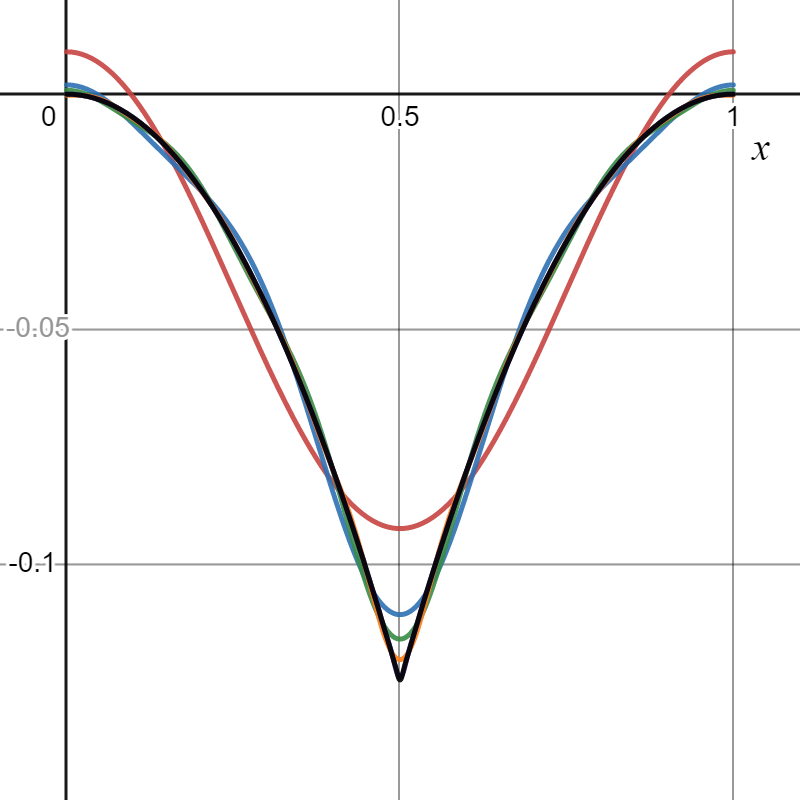
\includegraphics[width=0.5\textwidth]{figures/fundamental_solution.png}
\caption{Red curve is $N=1$, blue curve is $N=3$, green curve is $N=5$, orange curve is $N=10$, purple curve is $N=50$, and the black curve is $N=100$.}
\end{figure}
\item As you can see from large $N$ values, the true solution seems to have a cusp at $x=1/2$ and the true solution will have the correct boundary values. This cusp forms because is because that is the only place you are applying force. Since you are pressing on an elastic band, the whole band will deform, but since it is locked at the endpoints those will not move. Go ahead and try to mimic this experiment yourself if you can!
\end{enumerate}
\end{solution}
\vspace*{1cm}
\textcolor{red}{
\noindent \textbf{Rubric:}
\begin{enumerate}[(a)]
    \item \textbf{(1 pt.)} Integrate by parts with boundary condtions. \textbf{(1 pt.)} Got the correct result (up to a minus sign since my original problem had a typo).
	\item \textbf{(1 pt.)} Right idea in applying Fourier to both sides. \textbf{(1 pt.)} Correct result.
	\item \textbf{(1 pt.)} Correct Fourier series with $x_0$. \textbf{(1 pt.)} Correct series when $x_0=1/2$. 
	\item \textbf{(1 pt.)} Correct work to find $c_0$ and $c_1$.
	\item \textbf{(1 pt.)} All approximations are plotted. \textbf{(1 pt.)} Plot is on the correct domain.
	\item \textbf{(1 pt.)} Explanation of what the true answer is given the physical interpretation.
\end{enumerate}
}

\newpage
\begin{problem}
\textbf{(Bonus 10 pts.)} Show that the Fourier transform is an isomorphism between $\ell^2(\C)$ and $L^2(\Omega)$ where $\Omega=[0,1]$. For an extra 5 points, argue that this is true if $\Omega$ is any closed interval.
\end{problem}
\begin{solution}
This proof comes in a few parts. Let me write it out cleanly. Let me note that what I mean by isomorphism is that the Fourier transform
\[
\mathcal{F}\colon L^2(\Omega) \to \ell^2(\C)
\]
is an invertible linear map.
\begin{itemize}
\item First, note that the Fourier transform is (conjugate) linear since the inner product is (conjugate) linear, i.e.,
\[
\mathcal{F}(\alpha f+ \beta g) = \innprod{\alpha f + \beta g}{\phi_n} = \alpha^* \innprod{f}{\phi_n} + \beta^* \innprod{g}{\phi_n} = \alpha^* \mathcal{F}(f) + \beta^* \mathcal{F}(g).
\]
The fact that the constants receive a conjugate is just because I defined $\hat{f}(n)= \innprod{f}{\phi_n}$ instead of $\hat{f}(n)=\innprod{\phi_n}{f}$. This last bit is superficial and doesn't matter.

\item Next, note that the Fourier transform is invertible on its image since if I take $f(x)$ we have $\hat{f}(n) \in \operatorname{im}\mathcal{F}$. The inverse Fourier transform is the Fourier series since
\[
\mathcal{F}^{-1}(\hat{f}) = \sum_{n=-infty}^\infty \hat{f}(n) \phi_n(x) = f(x).
\]
Hence, at this point we know the Fourier transform is an invertible linear map.

\item The tough part is to show that the image of $\mathcal{F}$ is indeed $\ell^2(\C)$. A good enough argument for us is the following: Suppose that $f\in L^2(\Omega)$. Then we know 
\[
f(x) = \sum_{n=-infty}^\infty \hat{f}(n) \phi_n(x)
\]
by the previous part and moreover $f$ has finite energy so we have
\begin{align*}
\infty > \innprod{f}{f}_{L^2} &= \int_0^1 f^* f dx \\
&= \int_0^1 \left(\sum_{m=-infty}^\infty \hat{f}^*(m) \phi_m^*(x)\right) \left(\sum_{n=-infty}^\infty \hat{f}(n) \phi_n(x)\right) dx\\
&= \sum_{m=-\infty}^\infty \sum_{n=-\infty}^\infty \hat{f}^*(m)\hat{f}(n) \int_0^1 \phi_m^* \phi_n dx\\
&= \sum_{m=-\infty}^\infty \sum_{n=-\infty}^\infty \hat{f}^*(m)\hat{f}(n) \innprod{\phi_m}{\phi_n}\\
&= \sum_{m=-\infty}^\infty \sum_{n=-\infty}^\infty \hat{f}^*(m)\hat{f}(n) \delta_{mn}\\
&= \sum_{n=-\infty}^\infty \hat{f}^*(n)\hat{f}(n)\\
&= \sum_{n=-\infty}^\infty |\hat{f}(n)|\\
&= \innprod{\hat{f}}{\hat{f}}_{\ell^2}.
\end{align*}
Hence, we have found $\innprod{\hat{f}}{\hat{f}}_{\ell^2} < \infty$ which means that for any $f\in L^2(\Omega)$ the transform is an element of $\ell^2(\C)$. By the same work, given some sequence in $\ell^2(\C)$ you can build an $f \in L^2(\Omega)$ and thus we have proven the claim.
\end{itemize}

To extend this further, consider a new closed interval $[a,b]$. Now, this interval is \emph{topologically equivalent} to $[0,1]$ which is why this process will work. Anyhow, suppose we have $f(x)\in L^2([0,1])$. Then, consider an interval $[a,a+k]$ where $k>0$. Now, the function $f(x-a)\in L^2([a,a+1])$ by construction (we have just translated the input). Now, to create a function in $L^2([a,a+k])$ we can just take $\tilde{f}(x)=f(kx-a)$ and $\tilde{f}(x)\in L^2([a,a+k])$. This operation we have done to the input of $f$ is known as an \emph{affine transformation} and they are almost linear transformations! As a quick sanity check, $\tilde{f}(a)=f(0)$ and $\tilde{f}(a+k)= f(1)$. It is quite clear to see that if $f\in L^2([0,1])$ then
\[
\int_a^{a_k} \tilde{f}^* \tilde{f} dx < \infty.
\]
Hence, we can perform the Fourier transform on $[a,a+k]$ by undoing this, i.e., given $\tilde{f}(x)$ we can just take $f(x) = \tilde{f}(\frac{1}{k}x +a)$ and do the Fourier transform as we have learned. Then, to get back a Fourier transform on $[a,a+k]$ we can just apply our affine transformation to the $\phi_n$.
\end{solution}
\vspace*{1cm}
\textcolor{red}{
\noindent \textbf{Rubric:}
\begin{enumerate}[(a)]
    \item \textbf{(3 pt.)} Argue that the Fourier transform is (conjugate) linear in some way. \textbf{(3 pt.)} Use the Fourier series as an inverse. \textbf{(4 pt.)} Show that image of the Fourier transform is $\ell^2(\C)$ by showing work similar to mine. \textbf{(4 pt.)} Explaining how one can change the input to a function to get a function on a different interval. \textbf{(1 pt.)} Explain how this can be used with the Fourier transform.
\end{enumerate}
}



\end{document}